\chapter{Elemzés és tervezés}
\label{ch:spec}

\section{Kutatási cél}
\label{ch:goals}

A cél az, hogy a kutatás során szerzett modell megbízhatóan detektáljon hulladéklerakókat általánosan folyók mentén. Ehhez a false positive arányok minél kisebbek kell legyenek, míg a true positive arányok minél nagyobbak. Ugyanakkor nem jelent ugyanakkora problémát egy false negative, mint egy false positive, mivel a false positive eredmények fölöslegesen rossz irányba küldhetik a folyómentő csapatot. 
A kutatólabor 2023-as cikkjében bemutatott modell (továbbiakban meglevő modell) egyik problémája a nagy false positive arányok voltak. A modell a pusztazámori hulladéklerakóról, illetve a kiskörei víztárolóról szerzett adatokkal volt betanítva. Ezért érdemes első körben egy nagyobb adathalmazzal betanítani a modellt.

\section{Műhold specifikációk}

Az új Random Forest modell a PlanetScope műholdakra van specializálva, azon belül is a legújabb PSB.SD szenzorokra. A modell a Vörös (Red), Kék (Blue), Zöld (Green), és a közeli infravörös (NIR) sávokat használja. A PlanetScope műholdak körülbelül 3 méter/pixel felbontással rendelkeznek \cite{planetsensors2024}.

\section{Használt indexek}

A kutatás során felhasználom a kutatólaborban már számolt indexeket. Pontosabban a Plastic Index (\ref{eq:pi} képlet), Normalized Difference Water Index (\ref{eq:ndwi} képlet), Normalized Difference Vegetation Index (\ref{eq:ndvi} képlet), Reversed Normalized Difference Vegetation Index (\ref{eq:rndvi} képlet), Simple Ratio (\ref{eq:sr} képlet) indexek kerülnek használatra \cite{Themistocleous2020, magyar2023}.

\begin{equation}\label{eq:pi}
    Plastic \ Index \ (PI) = \frac{NIR}{NIR + Red}
\end{equation}

\begin{equation}\label{eq:ndwi}
    Normalized \ Difference \ Water \ Index \ (NDWI) = \frac{Green - NIR}{Green + NIR}
\end{equation}

\begin{equation}\label{eq:ndvi}
    Normalized \ Difference \ Vegetation \ Index \ (NDVI) = \frac{NIR - Red}{NIR + Red}
\end{equation}

\begin{equation}\label{eq:rndvi}
    Reversed \ Normalized \ Difference \ Vegetation \ Index \ (RNDVI) = \frac{Red - NIR}{Red + NIR}
\end{equation}

\begin{equation}\label{eq:sr}
    Simple \ Ratio \ (SR) = \frac{NIR}{Red}
\end{equation}

A Plastic Index, ahogy a neve is sugallja, egy olyan index, mely a vízen úszó hulladékok pixelein magas értékeket vesz fel, míg a vízpixeleken alacsony értékeket. A számításban kihasználásra kerül az, hogy a közeli-infravörös tartományban a hulladék sokkal jobban visszaverődik a vízhez képest, mint a vörös tartományban. Az NDWI a NIR és zöld sávokat használja fel a vízben található tárgyak, illetve növények kijelölésére \cite{McFeeters1996}. Az NDVI -1 és +1 értékek között tartózkodik. Ha adott területen az NDVI negatív értéket vesz fel, akkor nagy az esélyünk arra, hogy a terület az víz. Ha 1-hez közeli értéket vesz fel, akkor nagy eséllyel növényzet borítja az adott területet. Az RNDVI ennek a -1-szerese. A Simple Ratio is a vörös és közeli infravörös tartományokat használja ki a vegetáció további detektálásához és osztályozásához. 

\cite{Themistocleous2020}-ban összehasonlításra kerülnek ezek az indexek (\ref{fig:index-comparison} ábra): Összekötöttek több műanyag palackot, és felhelyezték a vízre. Ezután Sentinel-2 felvételekkel összehasonlították a különböző indexek teljesítményét ennek a szigetnek a megtalálásában. A kutatás eredménye az volt, hogy a Plastic Index tudta a legjobban kiemelni a műanyag-szigetet.

\begin{figure}[H]
	\centering
	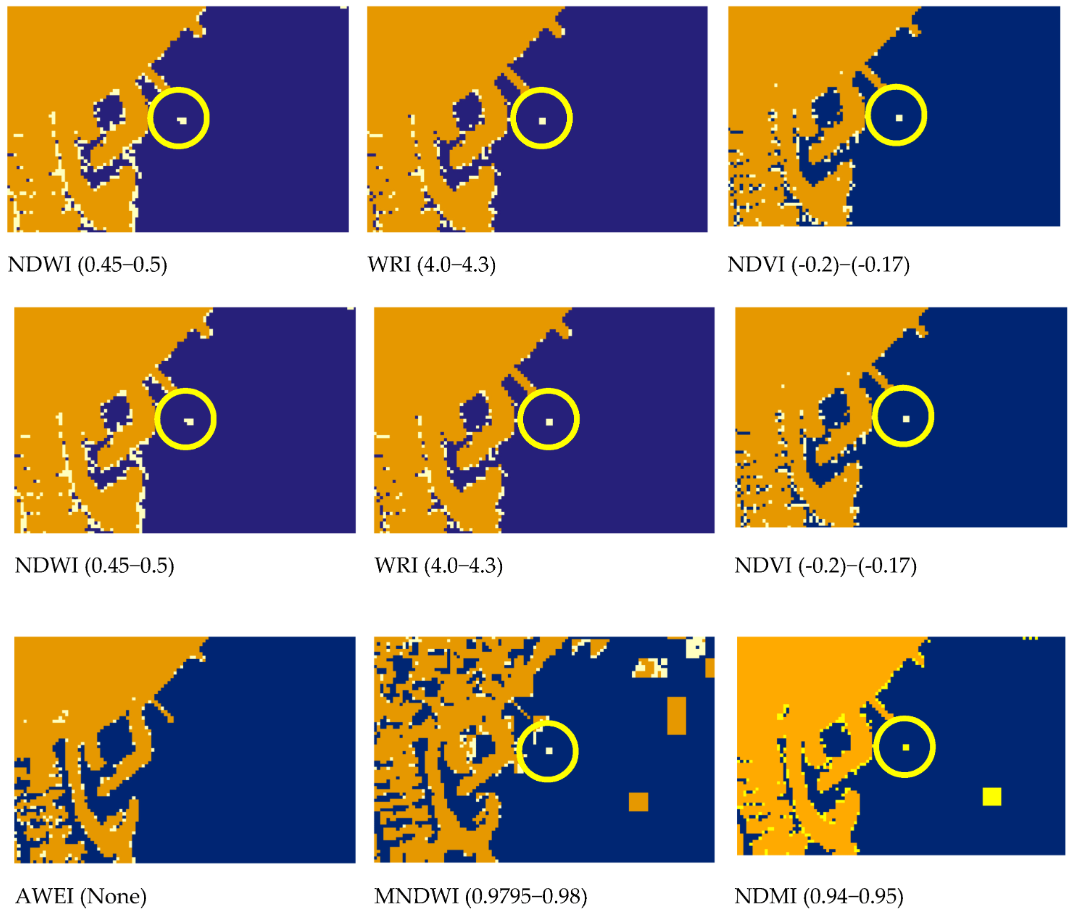
\includegraphics[width=0.6\textwidth,frame]{index-comparison}
	\caption{Különböző indexek összehasonlítása egy mesterségesen előállított úszó műanyag-palack szigeten \cite{Themistocleous2020}}
    \label{fig:index-comparison}
\end{figure}